\documentclass[10pt,a4paper]{article}
\usepackage[margin=1.9cm]{geometry}
\usepackage[T1]{fontenc}
\usepackage[utf8]{inputenc}
\usepackage[spanish,es-nodecimaldot]{babel}
\usepackage{lmodern,amsmath,amssymb,booktabs,graphicx,microtype}
\usepackage[hidelinks]{hyperref}
\setlength{\parindent}{0pt}
\setlength{\parskip}{5pt}
\newcommand{\R}{\mathbb R}
\newcommand{\Z}{\mathbb Z}
\begin{document}
\begin{center}
{\Large Verificación exacta con realimentación de cortes}\par
{\large Prueba acotada y decisión de cierre}\par
14 de octubre de 2026 --- Exploración separada de OMS v1.3.5
\end{center}

\textbf{Resultado.} Las dos variantes con cortes no mejoran el costo exactamente
respaldado de reparación ni del reinicio equivalente y añaden trabajo.
El control Base-B alcanza la calidad objetivo en seis de seis casos.
Se cierra este prototipo conforme al protocolo previo; no se modifica OMS.

\textbf{Diseño.} Un caso previamente seleccionado, \texttt{neos-3083784-nive},
4779 variables, 3240 binarias y 2836 filas; Gurobi 13.0.2 y HiGHS 1.15.1,
semillas nuevas 109,127,149, cuatro hilos, presolve/escalado interno habituales,
gap solicitado 1\%. Gurobi usa IntegralityFocus=1 en todos los brazos.
Las tolerancias normales son las mismas dentro de cada solver; Base-tight-B
las reduce a $10^{-9}$. Son 42 resultados y 60 llamadas MIP, no 42 llamadas.

A-numeric y B-repair comparten una llamada L2: A entrega el punto numérico;
B incorpora auditoría y reparación exacta con los enteros fijados.
B-restart y las dos C comparten una primera fase y su auditoría; después se
resuelven por separado. B-restart tiene reinicios y Starts equivalentes, sin cortes;
C-aggregate usa duales/rayos agregados, C-guard asignaciones binarias parciales.
Base-B y Base-tight-B conservan las filas originales sin L2 y verifican la salida.

\begin{center}\small
\begin{tabular}{llrrr}\toprule
Solver & Estrategia & Costo exacto $U$ & Meta & Mediana (s)\\\midrule
Gurobi & A-numeric & sin certificar & 0/3 & 0.242 \\
Gurobi & B-repair & 50001/53331/74091 & 0/3 & 1.359 \\
Gurobi & B-restart & 50001/53331/74091 & 0/3 & 2.923 \\
Gurobi & C-aggregate & 50001/53331/74091 & 0/3 & 4.208 \\
Gurobi & C-guard & 50001/53331/74091 & 0/3 & 4.145 \\
Gurobi & Base-B & 27851 & 3/3 & 1.732 \\
Gurobi & Base-tight-B & 27851 & 3/3 & 1.614 \\
HiGHS & A-numeric & sin certificar & 0/3 & 0.239 \\
HiGHS & B-repair & -- & 0/3 & 1.007 \\
HiGHS & B-restart & -- & 0/3 & 2.045 \\
HiGHS & C-aggregate & -- & 0/3 & 3.683 \\
HiGHS & C-guard & -- & 0/3 & 3.632 \\
HiGHS & Base-B & 27851 & 3/3 & 5.683 \\
HiGHS & Base-tight-B & 29651/29651/29311 & 0/3 & 31.319 \\
\bottomrule\end{tabular}
\end{center}
\textbf{Lectura.} $U$ es un testigo racional factible con conversión flotante
comprobada; los tres costos siguen 109/127/149. ``--'' indica ausencia de testigo
obtenido, no inviabilidad global. La meta $U\le28129.51=1.01(27851)$ usa solo
un escalar factible previo, sin importar su punto o certificados. No es una
prueba de optimalidad. A informa cero nominal en 6/6, sin respaldarlo exactamente.
Los segundos incluyen importación, cotejo, auditoría y realimentación; la
auditoría retrospectiva de A es evaluación externa, no trabajo de A.

\newpage
\textbf{Qué se pudo transferir a otros patrones.}
Todas las cotas continuas se incorporan como filas, con variables continuas libres.
Para $Ay\le b-Bz$, un dual $\pi\le0$, $A^\top\pi=c_C$, da
$g(z)=\pi^\top(b-Bz)$ y el corte $c_C^\top y\ge g(z)$.
Un rayo $r\le0$, $A^\top r=0$, da $r^\top(b-Bz)\le0$.
Son construcciones clásicas de Benders. En este modelo monolítico, sus agregados
son redundantes en aritmética exacta; no se implementó un maestro descompuesto.

Para binarias se conserva un subconjunto $S$ que garantiza
$\min\{g(z):z_S=z_S^k,\ 0\le z\le1\}\ge V$.
Con un piso global continuo $L\le V$ se obtiene el corte válido
\[
 c_C^\top y\ \ge\ V-(V-L)
 \left[\sum_{i\in S:z_i^k=0}z_i+\sum_{i\in S:z_i^k=1}(1-z_i)\right].
\]
Se liberan sin pérdida los índices ya situados en su extremo minimizador de $g$.
Los diez certificados factibles heredados y los tres nuevos reducen $S$ a
\textbf{20 binarias}, de 3240. El piso vale para cualquier continuación de la
asignación parcial; no es su costo exacto ni prueba su factibilidad.

Para un rayo, si el mínimo de $r^\top(b-Bz)$ con $z_S=z_S^k$ sigue positivo,
la misma suma entre corchetes debe ser al menos uno. Se liberan decisiones
por pérdida creciente de margen mientras se preserve esa prueba. Los dos
conflictos heredados usan 26 y 28 decisiones; los nueve nuevos, entre 25 y 45.
La validez global se comprueba con identidades exactas y soporte de caja,
sin enumerar exclusivamente patrones observados. Son técnicas de Benders
lógico/entero conocidas; no se afirma novedad de esas desigualdades [1,2].

\begin{center}
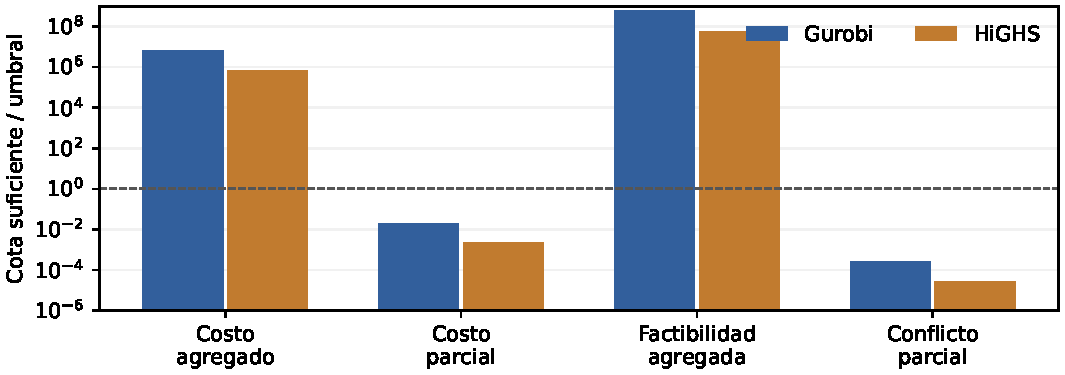
\includegraphics[width=.88\linewidth]{cut-transfer.pdf}
\end{center}
\textbf{Figura.} Máximo sobre los 24 cortes heredados. Cota condicional del
residuo tras redondear enteros, dividida por 1\% del piso de costo o por una
unidad para factibilidad. Menor que uno es suficiente bajo las hipótesis;
mayor que uno no predice una violación. Se usa $\gamma=10^{-5}$ en Gurobi,
$10^{-6}$ en HiGHS y residuo exportado $10^{-6}$. El soporte pequeño mejora
esta cota, pero \textbf{no produjo una mejora de calidad en el ensayo}.

\newpage
\textbf{Exactitud de exportación, auditoría y atribución.}
Los presupuestos de aceptación de las filas originales son
$\delta_i=10^{-4}\max(1,|b_i|)$, con presupuesto de cotas $10^{-4}$ e
integralidad exacta al certificar. Son elecciones algebraicas experimentales,
no tolerancias físicas del despacho. Se conserva el modelo binary64 original,
cotejado con el MPS, incluidos objetivo, dominios y cotas. L2 es diádico.

Cada corte se escala por una potencia de dos con coeficientes en
$[10^{-9},10^9]$. El residuo exportado $10^{-6}$ debe corresponder como máximo
a una unidad de costo o 0.25 unidades de una fila primitiva de factibilidad.
Si se redondea $\alpha a$ a $\widehat a$, se calcula exactamente
$R=\max_{x\text{ en caja original}}(\alpha a-\widehat a)^\top x$
y se exporta $\widehat b\le\alpha b-R$, redondeado hacia abajo para el sentido
$\ge$. Esto evita fortalecer por error el corte; una cota necesaria no acotada
provoca abstención. Se cotejan coeficientes y RHS tras importar al solver.
Los 24 cortes nuevos pudieron exportarse con prueba de debilitamiento seguro.

Para una fila exacta $a^\top x\ge b$, respetar el residuo exportado no elimina
la contribución de redondear enteros. Bajo las hipótesis comprobadas,
\[
 (b-a^\top(\bar z,y))_+
 \ \le\ \epsilon/\alpha+\text{defecto de exportación}
       +\gamma\sum_{i\text{ entero}}|a_i|.
\]
Es una cota suficiente, no necesaria. Los grandes coeficientes agregados
debilitan su utilidad; las cláusulas cortas mejoran el margen.

\textbf{Verificación independiente.} Se reconstruyeron los LP y verificaron
51 certificados nuevos: 18 óptimos con testigo y 33 rayos de inviabilidad;
hubo nueve accesos a cache. Se auditaron 44 patrones distintos, 30 inviables.
Los patrones inviables aparecen 42 veces en las salidas nativas. Son
apariciones, no 42 patrones distintos. La cache es local a cada estrategia;
se comprueba que los cortes solo usan pruebas disponibles previamente,
los Starts equivalentes y la retención del mejor testigo exacto.

En las \textbf{36 observaciones de cortes activos} no se detectaron violaciones
del corte exacto después de redondear enteros, ni incumplimientos del residuo
exportado o de $\gamma$. Ambas C siguieron produciendo patrones inviables
distintos: la información aprendida no cubría todos los patrones problemáticos.
No corresponde atribuir el resultado negativo a violaciones observadas de cortes.

\textbf{Gaps y estados.} Las 48 llamadas L2 etiquetadas óptimas entregaron
costo nominal cero. Seis tienen patrón con costo exacto mínimo positivo; las
otras 42 apariciones tienen patrón sin continuación exacta. La evaluación
del objetivo del punto numérico es correcta: lo que falta es respaldo exacto
para su patrón. No se encontraron contradicciones independientes entre una
cota inferior reportada y un mejor testigo exacto. El mejor costo exacto
27851 es una cota superior, \textbf{sin certificado de optimalidad MILP global}.
No se refutaron de forma independiente 48 afirmaciones de gap global.

\textbf{Trabajo.} Ambas C y B-restart tienen hasta tres fases de 10 s;
A/B y cada Base tienen hasta 30 s en una llamada. Se usa parada por objetivo
nominal, pero el procedimiento solo declara éxito con $U$ exacto.
Igual máximo solicitado no significa igual trabajo realizado. Referencia de
ciclo 45 s, ajustada tras importar; no hubo excesos ni errores de ejecución.
Preparación compartida: 0.014 s, informada aparte. Los prefijos compartidos
se cobran íntegramente a cada estrategia, no son réplicas independientes.

\newpage
\textbf{Decisión y alcance.}
En los doce pares C frente a B-restart (dos familias, dos solvers, tres semillas)
hubo cero mejoras del mejor $U$ y cero ganancias en la meta. C tampoco mejora
el costo de B-repair. Añade construcción, comprobación y nuevas auditorías.
Base-B alcanza la meta en 6/6; Base-tight-B la alcanza en Gurobi, mientras
HiGHS consume 30 s y termina con $U=29651,29651,29311$.
No se sostiene que endurecer tolerancias mejore siempre el resultado.

Se cierra esta realimentación monolítica con máximo de tres fases, sin añadir
semillas, modelos o iteraciones para buscar una ventaja. Un modelo seleccionado
por anomalías previas y tres semillas no justifican inferencia poblacional.
El resultado tampoco descarta otras políticas o una descomposición Benders real.
\textbf{No se incorpora material al artículo OMS ni se altera su versión v1.3.5.}

\textbf{Qué queda de las otras líneas.}
La nota separada \texttt{NOTA\_PREVENTIVA.md} deriva condiciones suficientes
uniformes para patrones desconocidos: familias completas de vértices duales
para costo y rayos de Farkas normalizados para exclusión de patrones inviables.
La racionalidad da un margen de retícula, pero la existencia de presupuestos
positivos no demuestra que sean calculables con costo razonable o utilizables
con tolerancias del solver. El banco parcial de este ensayo no cumple esa
hipótesis de completitud. No se presenta el argumento como un teorema nuevo;
existen cotas de Hoffman y cotas de error mixtas pertinentes [3,4].

\texttt{QUE\_SIGUE.md} delimita una eventual prueba de selección de cortes en
un maestro Benders real del despacho. Geometría y ortogonalidad por sí solas
ya tienen antecedentes [5,6]. Haría falta una mejora frente a selectores fuertes,
contabilizando resolver maestro/subproblemas y conservar la misma garantía.
Aquí no se modificó C++ ni se ejecutó ese experimento. La certificación racional
general tampoco se ofrece como novedad: SCIP dispone de modo exacto y VIPR [7].

\textbf{Reproducción y material.}
\texttt{README.md} documenta comandos; \texttt{PROTOCOL.md}, \texttt{design.json}
y cinco snapshots fijan el procedimiento anterior a las nuevas resoluciones.
El paquete incluye entradas, 60 salidas nativas y logs, pruebas racionales,
CSV, verificador independiente, seis tests y fuentes de esta nota/figura.
El replay comprueba las pruebas sin llamar solvers; ejecutar de nuevo los solvers
requiere instalaciones/licencias y no garantiza tiempos o trayectorias idénticos.
\texttt{MANIFEST.json} inventaría el ZIP; \texttt{VALIDATION.json} registra replay
desde extracción limpia, hashes, recompilación y conservación de OMS y cinco
paquetes anteriores. Los binarios y licencias de solvers quedan fuera.

\small
\textbf{Referencias primarias consultadas.} Son antecedentes, no comparaciones
de rendimiento efectuadas en este trabajo.

[1] Hooker, \emph{Logic-Based Benders Decomposition}.
\url{https://arxiv.org/abs/1910.11944}.

[2] Laporte y Louveaux, \emph{The integer L-shaped method} (1993).
\url{https://doi.org/10.1016/0167-6377(93)90002-X}.

[3] Peña, Vera y Zuluaga, \emph{New characterizations of Hoffman constants}.
\url{https://arxiv.org/abs/1905.02894}.

[4] Stein, \emph{Error bounds for mixed integer linear optimization problems}.
\url{https://doi.org/10.1007/s10107-015-0872-7}.

[5] Hosseini y Turner, \emph{Deepest Cuts for Benders Decomposition}.
\url{https://arxiv.org/abs/2110.08448}.

[6] Glomb, Liers y Rösel, \emph{A novel Pareto-optimal cut selection strategy}.
\url{https://doi.org/10.1007/s12532-025-00291-1}.

[7] SCIP 10, modo exacto y certificados VIPR.
\url{https://scipopt.org/doc-10.0.0/html/EXACT.php}.
\end{document}
